\subsection{Bayesian Neural Networks}

%When implementing an intelligent search, it is desirable to utilize a predictive method as a fast approximation to either an expensive calculation, or an experimentally observed value.  Additionally, since the goal is the large scale exploration of chemical space, the method must also possess good scaling characteristics.  In this regard, neural networks provide an ideal solution.  

Neural networks are well-suited for our purposes.
They produce state-of-the-art results when predicting chemical properties of molecules \cite{Ma_2015,Mayr_2016,ramsundar2015massively} and can be applied to large data sets by using stochastic optimization techniques \cite{bousquet2008tradeoffs}. However, common applications of neural networks focus only on the deterministic prediction scenario. In our case, for successful exploration, it is desirable to use a probabilistic prediction paradigm. While making probabilistic predictions with neural networks is traditionally a difficult task, we use here a recent breakthrough in scalable training of Bayesian neural networks known as probablistic back-propagation (PBP) \cite{hernandez2015probabilistic}. 

Given data~${\mathcal{D} = \{\mathbf{x}_n, y_n \}_{n=1}^N}$, formed by feature vectors~${\mathbf{x}_n \in \mathbb{R}^D}$ and targets~${y_n \in \mathbb{R}}$, we assume that~${y_n = f(\mathbf{x}_n;\mathcal{W}) + \epsilon_n}$,
where~$f(\cdot ;\mathcal{W})$ is the output of a neural net with weights $\mathcal{W}$. The network output is corrupted by additive noise variables~$\epsilon_n \sim \mathcal{N}(0,\gamma^{-1})$. The network has~$L$ layers, with~$V_l$ hidden units in layer~$l$, and~${\mathcal{W} = \{ \mathbf{W}_l \}_{l=1}^L}$ is the collection of~${V_l \times (V_{l-1}+1)}$ weight matrices. The $+1$ is introduced here to account for the additional per-layer biases. The activation functions for the hidden layers are rectifiers: ${\varphi(x) = \max(x,0)}$. Let $\mathbf{y}$ be an $N$-dimensional vector with the targets~$y_n$ and~$\mathbf{X}$ be an ${N\times D}$ matrix of feature vectors~$\mathbf{x}_n$. The entries of the matrices in $\mathcal{W}$ are \emph{a priori} distributed according to a Gaussian distribution with zero mean and variance $\lambda^{-1}$. The priors on $\gamma$ and $\lambda$ are Gamma distributions with small shape and rate parameters.

PBP approximates the posterior distribution on $\mathcal{W}$, $\gamma$ and $\lambda$ with the tractable distribution
\begin{equation}
q(\mathcal{W},\gamma, \lambda) = \left[ \prod_{l=1}^L\! \prod_{i=1}^{V_l}\! 
\prod_{j=1}^{V_{l\!-\!1}\!+\!1} \mathcal{N}(w_{ij,l}| m_{ij,l},v_{ij,l})\right ]
 \text{Gam}(\gamma \,|\, \alpha^\gamma, \beta^\gamma)
\text{Gam}(\lambda \,|\, \alpha^\lambda, \beta^\lambda)\,.\label{eq:posterior_approximation}
\end{equation}
PBP tunes the parameters of $q$ by iterating an assumed
density filtering (ADF) algorithm over the training data \cite{opper1998bayesian}. The main operation in PBP
is the update of the mean and variance parameters of (\ref{eq:posterior_approximation})
each time a new data point is processed. 

\begin{figure}[hb]
\centering
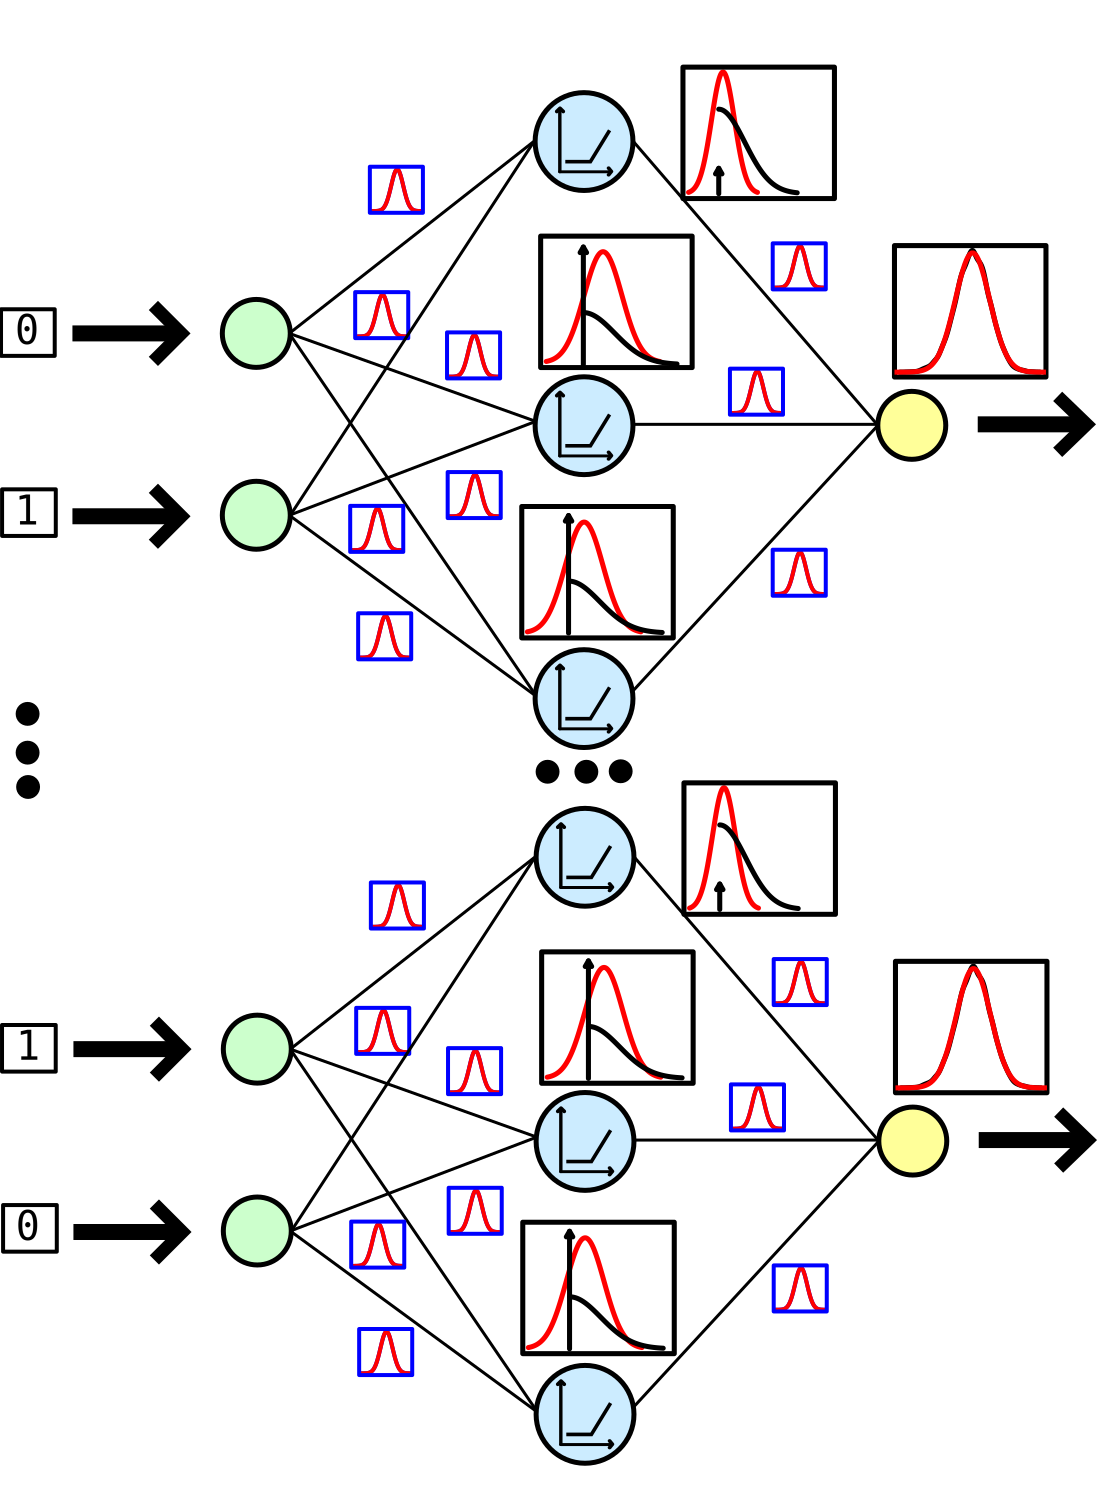
\includegraphics[width=0.8\columnwidth]{figures/pbp.png}

\caption{A graphical representation of the probabalistic back propagation (PBP) algorithm. Deterministic inputs, here represented as $1$s and $0$s are passed through the Bayesian neural network. The main operation in PBP is the update of the mean and variance parameters of the posterior approximation each time a new data point is processed. Updates are propagated using moment matching between the old and new liklihoods, with ADF Gaussian updates.}
\label{fig:pbp}
\end{figure} 
For this, PBP matches moments between
the new $q$ and the product of the old $q$ and the likelihood factor
$\mathcal{N}(y_n\given f(\mathbf{x}_n;\mathcal{W}),\gamma^{-1})$,
where $f(\mathbf{x}_n;\mathcal{W})$ denotes the output of the network for input $\mathbf{x}_n$ and weight values $\mathcal{W}$.
The matching of moments for the weights is achieved by using standard ADF Gaussian updates (see
\cite{minka2001family}, equations 5.12 and 5.1):
\begin{align}
m_{ij,l}^\text{new} & = m_{ij,l} + v_{ij,l} \nabla_{m_{ij,l}} \log Z \,,\label{eq:adf_update_1}\\
v_{ij,l}^\text{new} & = v_{ij,l} - v_{ij,l}^2 \left[ (\nabla_{m_{ij,l}} \log Z)^2 - 2 \nabla_{v_{ij,l}} \log Z \right]\,,\label{eq:adf_update_2}
\end{align}
where $Z$ is the result of marginalizing the likelihood $\mathcal{N}(y_n\given f(\mathbf{x}_n;\mathcal{W}),\gamma^{-1})$ with
respect to $q$. The computation of $Z$ is intractable. However, PBP circumvents this problem by
approximating the distribution of the network output $f(\mathbf{x}_n;\mathcal{W})$ when $\mathcal{W} \sim q$ with a Gaussian. 
This is achieved in a forward pass through the network where each non-Gaussian distribuion
for the output of each neural unit is approximated with a Gaussian by moment matching.
When $\gamma\sim q$, the marginalization of $\mathcal{N}(y_n\given f(\mathbf{x}_n;\mathcal{W}),\gamma^{-1})$ 
with respect to $\gamma$ produces a Student's $t$ density which does not
convolve in closed form with respect to the Gaussian approximation on $f(\mathbf{x}_n;\mathcal{W})$. Neverheless, this Student's
$t$ density can be as well approximated with a Gaussian by moment matching to obtain a closed form convolution that approximates $Z$.
The gradients required in (\ref{eq:adf_update_1}) and (\ref{eq:adf_update_2}) can then be obtained by backpropagation.
After several ADF iterations over the data,  we can obtain a probabilistic
prediction for $f(\mathbf{x}_\star;\mathcal{W})$ given the test input
$\mathbf{x}_\star$ by applying the forward pass process described above.  We
refer the reader to \cite{hernandez2015probabilistic} for full details on PBP; a graphical depiction of the process of training a Bayesian neural network using PBP is shown in Figure \ref{fig:pbp}.

